% ju 17-Jul-22
\documentclass[a4paper,12pt,fleqn,parskip=half]{scrartcl}
\usepackage[ngerman]{babel}
\usepackage[utf8]{inputenc}
\usepackage[T1]{fontenc}

% Schrift
%\usepackage{lmodern}
\usepackage[osf,sc]{mathpazo} 
\usepackage[scale=.9,semibold]{sourcecodepro}   
\usepackage[osf]{sourcesanspro}  

\usepackage[headsepline]{scrlayer-scrpage}
\pagestyle{scrheadings}
\clearpairofpagestyles

\usepackage[table,dvipsnames,usenames]{xcolor}
\usepackage{textcase}
\usepackage{nameref}
\usepackage{hyperref}
\usepackage{tabularx}
\usepackage{multirow}
\usepackage{multicol}
\usepackage{caption, booktabs}
\usepackage{graphicx} 
\usepackage{scrhack}    
\usepackage{url}%% Links
\usepackage[inline]{enumitem}
\usepackage{pifont}
\usepackage{eurosym}% \euro 20,-
\usepackage{amsmath}
\usepackage{amsfonts}
\usepackage{amssymb}
\usepackage{array}            % Extending the array and tabular environments
\usepackage{chngcntr}         % Change the resetting of counters
\usepackage[version=4]{mhchem}
\usepackage{stmaryrd}
\usepackage{siunitx}
\usepackage{float}
\usepackage{csquotes}
\usepackage{subcaption}
\usepackage{mathtools}
\usepackage{icomma}%Dezimaltrennzeichen
\usepackage{multimedia}%Video: \movie[externalviewer]{(video.mov)}{video.mov}
\usepackage{epstopdf}
\usepackage{footnote}
\usepackage{qrcode}% Anwendung: \qrcode[hyperlink,level=Q,version=2,height=1cm]{\website}
\usepackage{underscore}% Unterstrich ____

% PDF Dokumente einbinden
\usepackage{pdfpages}% \includepdf[pages=-]{Tabellen/Excel.pdf}
\RequirePackage{lastpage}  % Pagecounter

\addto\captionsngerman{%
\renewcommand{\figurename}{Abb.}
\renewcommand{\tablename}{Tab.}
}

% listings
\usepackage{listings}
\lstset{basicstyle=\linespread{1}\ttfamily\small,floatplacement=!htb,captionpos=t,abovecaptionskip=.5\baselineskip,belowcaptionskip=.5\baselineskip,upquote=true,showstringspaces=false,inputencoding=utf8,tabsize=4,
    	keywordstyle=\bfseries ,
	commentstyle=\color{rot5},
	stringstyle=\color{orange},
	breaklines=true,
  	postbreak=\mbox{\textcolor{black}{$\hookrightarrow$}\space},
	breakatwhitespace=false
}
\lstset{literate={á}{{\'a}}1 {é}{{\'e}}1 {í}{{\'i}}1 {ó}{{\'o}}1 {ú}{{\'u}}1 {Á}{{\'A}}1 {É}{{\'E}}1 {Í}{{\'I}}1 {Ó}{{\'O}}1 {Ú}{{\'U}}1 {à}{{\`a}}1 {è}{{\`e}}1 {ì}{{\`i}}1 {ò}{{\`o}}1 {ù}{{\`u}}1 {À}{{\`A}}1 {È}{{\'E}}1 {Ì}{{\`I}}1 {Ò}{{\`O}}1 {Ù}{{\`U}}1 {ä}{{\"a}}1 {ë}{{\"e}}1 {ï}{{\"i}}1 {ö}{{\"o}}1 {ü}{{\"u}}1 {Ä}{{\"A}}1 {Ë}{{\"E}}1 {Ï}{{\"I}}1 {Ö}{{\"O}}1 {Ü}{{\"U}}1 {â}{{\^a}}1 {ê}{{\^e}}1 {î}{{\^i}}1 {ô}{{\^o}}1 {û}{{\^u}}1 {Â}{{\^A}}1 {Ê}{{\^E}}1 {Î}{{\^I}}1 {Ô}{{\^O}}1 {Û}{{\^U}}1 {œ}{{\oe}}1 {Œ}{{\OE}}1 {æ}{{\ae}}1 {Æ}{{\AE}}1 {ß}{{\ss}}1 {ű}{{\H{u}}}1 {Ű}{{\H{U}}}1 {ő}{{\H{o}}}1 {Ő}{{\H{O}}}1 {ç}{{\c c}}1 {Ç}{{\c C}}1 {ø}{{\o}}1 {å}{{\r a}}1 {Å}{{\r A}}1 {€}{{\EUR}}1 {£}{{\pounds}}1 {~}{{\textasciitilde}}1 {-}{{-}}1 }

% bibliography
\usepackage[
    bibencoding=utf8,
    backend=biber,% bibtex, biber
    backref=false,backrefstyle=three+,url=true,urldate=comp,abbreviate=false,maxnames=20
]{biblatex} %Paket laden
\DeclareBibliographyCategory{cited}
\let\defaultcite\cite\renewcommand*\cite[2][]{\addtocategory{cited}{#2}\defaultcite[#1]{#2}}
\let\defaulttextcite\textcite\renewcommand*\textcite[2][]{\addtocategory{cited}{#2}\defaulttextcite[#1]{#2}}
\setcounter{biburllcpenalty}{7000}
\setcounter{biburlucpenalty}{8000}
\AfterPackage{biblatex}{
	\PreventPackageFromLoading[\errmessage{Sie haben versucht, das Cite-Paket zu laden, das nicht mit biblatex kompatibel ist.}]{cite}
}

\hypersetup{%
	%pdftitle={\titel},
	%pdfsubject={Latex},
	%pdfauthor={\autor},
	%pdfcreator={\autor}, 
	bookmarksnumbered=true,
	breaklinks=true,
	%colorlinks=true,	   
	linkcolor=rot5,		
	filecolor=blau5,		
	urlcolor=blau5,			
	citecolor=ForestGreen
}

\linespread{1.1}
\setlist{itemsep=0pt}
\widowpenalty10000
\clubpenalty10000
\tolerance1000   

\usepackage[left=2cm,right=2cm,top=1cm,bottom=1cm,includeheadfoot]{geometry}
%\usepackage[left=4cm,right=2cm,top=1cm, bottom=1cm,includeheadfoot]{geometry}
%\usepackage[left=6cm,right=1cm,top=1cm, bottom=1cm,includeheadfoot]{geometry}
%\usepackage[landscape=true,left=2cm,right=2cm,top=1cm,bottom=1cm,includeheadfoot]{geometry}%quer

% eigene Farbe definieren
% Adobe Prozessfarben: CMYK: 100,50,0,35 -> 1,0.5,0,0.35
\definecolor{orange}{cmyk}{0,0.55,0.61,0}   % 0,55,61,0
\definecolor{blau5}{cmyk}{1,0.77,0.1,0.01}  % 100,77,10,
\definecolor{rot5}{cmyk}{0.22,1,1,0.19}     % 22,100,100,19
\definecolor{grau2}{cmyk}{0,0,0,0.1}        % 0,0,0,40
\definecolor{blau}{cmyk}{0.93,0.66,0,0.21}% 

% Literatur
\bibliography{content/literatur}
\bibliography{content/literatur-kfz}
\bibliography{content/literatur-sport}

%%%%%%%%%%%%%%%%%%%%%%%%%%%%%%%%%%%%%%%%%%%%%%%%%%%%%%%
\newcommand{\name}{Jan Unger}
\newcommand{\thema}{01-Kostenrechnung}
\newcommand{\quelle}{\name}
\newcommand{\website}{https://bw-ju.de/}
\newcommand{\github}{https://github.com/ju1-eu}
%%%%%%%%%%%%%%%%%%%%%%%%%%%%%%%%%%%%%%%%%%%%%%%%%%%%%%%

\ihead{\textbf{Quelle:} \quelle}%{Kopfzeile innen}
\ohead{\textbf{Datum:} \today}  %{Kopfzeile außen}
\ifoot{\textbf{Thema:} \thema}  %{Fußzeile  innen}
\ofoot{Seite {\thepage} von {\pageref{LastPage}}}%{Fußzeile  außen}

\title{\thema}
\author{\name}
\date{\today}

\begin{document}
	%%%%%%%%%%%%%%%%%%%%%%%%%%%%%%%%%%%%%%%%%%%%%%%%%%%%%%%%%%%%%%%%%%
	\begin{abstract}
		\center
		\textbf{\Large \thema}%14pt
		
		\vspace{1.5em}
		%\datum	
		%\qrcode[hyperlink,level=Q,version=2,height=1cm]{\website}
		\qrcode[hyperlink,level=Q,version=2,height=1cm]{\github}
		
		\vspace{1.5em} 
		\raggedright
		\textbf{\large Keywords}
		% Checkliste
		\begin{itemize}[label=\checkmark]
			\item Begriff
		\end{itemize}
	\end{abstract}
    %%%%%%%%%%%%%%%%%%%%%%%%%%%%%%%%%%%%%%%%%%%%%%%%%%%%%%%%%%%%%%%%%%

	% anpassen
	%\input{content/tex/neu}
	%ju 28-Mai-22 01-Kostenrechnung.tex
$\to$ \emph{Ziel:} Kenngrößen verbessern (Produktivität,
Wirtschaftlichkeit, Umsatzrentabilität)

\textbf{Kosten- und Leistungsrechnung} (KLR) $\to$ internes
Rechnungswesen

vs.

\textbf{Buchhaltung} (FiBu) $\to$ externes Rechnungswesen

\textbf{Kosten einteilen}

\begin{enumerate}
\item
  \textbf{Vollkostenrechnung}

  \begin{itemize}
  \item
    Indirekte Kosten (Gemeinkosten, kalkulatorische Kosten)
  \item
    Direkte Kosten (Einzelkosten)
  \end{itemize}
\item
  \textbf{Kostenstellenrechnung} (Verursachergerechte Verteilung der
  Kosten: Lager, Werkstatt, Vertrieb)
\item
  \textbf{Teilkostenrechnung} (fixe Kosten, variable Kosten,
  Deckungsbeitrag)
\end{enumerate}

\section{Vollkostenrechnung}\label{vollkostenrechnung}

Vgl. Kostenrechnung Fachbuch S. 79-102
(\textcite{heiser:2017:betriebsfuhrung}).

\subsection{Kosten der Werkstatt}\label{kosten-der-werkstatt}

\begin{figure}[!ht]% hier: !ht
\centering
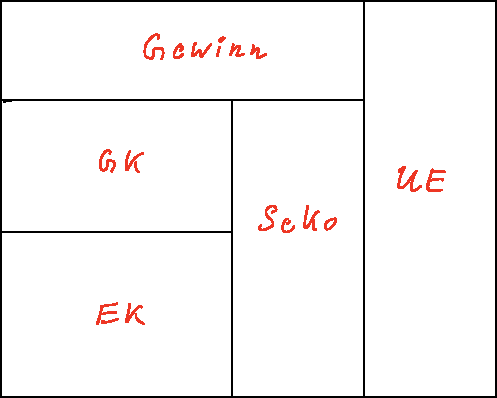
\includegraphics[width=0.4\textwidth]{images/Skizze/02_Umsatzerloese_Skizze.pdf}
\caption{Kosten und Erlöse}
%\label{fig:}%% anpassen
\end{figure}

\begin{enumerate}
\item
  \textbf{Einzelkosten} (EK), direkte Kosten (Kunden), Fertigungslöhne
  $\to$ produktive Löhne

  \begin{itemize}
  \item
    \emph{Beispiel:} Fertigungslöhne, Anschaffungskosten,
    Fertigungsmaterialien (Ersatzteile)
  \item
    $\boxed{\text{FL} = WSL \cdot Flh}$\\
  \item
    (WSL) = (StLs) Werkstattschnittlohn = Stundenlohnsatz
  \end{itemize}
\item
  \textbf{Gemeinkosten} (GK), indirekte Kosten, Hilfslöhne (W-Aufträge)
  $\to$ unproduktive Löhne

  \begin{itemize}
  \item
    $\boxed{\text{GK} = Seko - EK} \quad \boxed{\text{GK} = \frac{WSL \cdot GKZs}{100}}$
  \end{itemize}
\item
  \textbf{Selbstkosten} (SeKo)

  \begin{itemize}
  \item
    $\boxed{SeKo = EK + GK}$ (Einzelkosten + Gemeinkosten)
  \item
    $\boxed{SeKo = FL + GK}$ vs.~$\boxed{SeKo/h = WSL + GK/h}$
  \item
    $\boxed{SeKo_{EUR} = UE - GW} \to \boxed{SeKo_\% = 100~\% - UR_\%}$
  \end{itemize}
\item
  \textbf{Gewinn} (GW) in €

  \begin{itemize}
  \item
    $\boxed{\text{Gewinn} = UE - EK - GK} \quad \boxed{\text{Gewinn/h} = StVs - Seko/h}$
  \end{itemize}
\item
  \textbf{Umsatzerlöse} (UE in EUR), Stundenverrechnungssatz (StVs in
  EUR/h)

  \begin{itemize}
  \item
    Betrag für eine Leistung = Kostendecken + Gewinn
  \item
    $\boxed{UE = EK + GK + GW} \quad \boxed{UE = Seko + GW}$
    (Selbstkosten + Gewinn)
  \item
    $\boxed{StVs = StLs/WSL + GK + GW}$
  \end{itemize}
\end{enumerate}

\subsection{Gemeinkosten}\label{gemeinkosten}

\emph{Beispiel:}

\begin{itemize}
\item
  Lohn+Gehalt (unproduktiv)
\item
  Reisekosten
\item
  Kfz (geschäftlich)
\item
  Afa
\item
  Eigenkapital (EK \% Zins)
\item
  kalkulatorische Pacht
\item
  Meisterlohn (unproduktiv)
\item
  kalkulatorische Lohn (Frau)
\end{itemize}

\begin{enumerate}
\item
  \textbf{Gemeinkostenzuschlagsatz} (GKZs) in \%

  \begin{itemize}
  \item
    $\boxed{\text{GKZs} = \frac{GK \cdot 100}{FL}}$
  \end{itemize}
\item
  \textbf{Kalkulatorische Kosten} Gemeinkosten, die keine Ausgaben
  verursachen; aufwandsfremde Kosten

  \begin{itemize}
  \item
    \emph{Beispiel:} kalk.-Miete, kalk.-Abschreibungen, kalk.-Zinsen,
    kalk.-U-Lohn, kalk.-Wagnisse
  \end{itemize}
\item
  \textbf{Hilfslöhne} entstehen bei Werkstattaufträgen (W-Aufträge)

  \begin{itemize}
  \item
    \emph{Beispiel:} Leerlauf, Nacharbeiten, Reparatur von
    Werkstattfahrzeuge, Urlaub, Feiertage, Wartezeiten
  \end{itemize}
\end{enumerate}

\subsection{Gewinn}\label{gewinn}

Einkommen des Unternehmers, Wagnis, Unternehmensrisiko

\textbf{Gewinnzuschlag} (GWZs) in \%
$\boxed{\text{GWZs} = \frac{GW \cdot 100}{SeKo}}$

\newpage

\subsection{Fertigungslöhne}\label{fertigungsloehne}

\begin{enumerate}
\item
  \textbf{Fertigungslöhne} (FL), >>produktiv<<, EK, direkt

  \begin{itemize}
  \item
    Auftrag direkt dem Kunden in Rechnung stellen
  \item
    $\boxed{\text{FL} = WSL \cdot Flh}$
  \item
    \emph{Beispiel:} $90~\%$ Lohnkosten
  \end{itemize}
\end{enumerate}

$+$

\begin{enumerate}
\setcounter{enumi}{1}
\item
  \textbf{Hilfslöhne} (HL) >>unproduktiv<<, GK, nicht direkt

  \begin{itemize}
  \item
    \emph{Beispiel:} $10~\%$ Lohnkosten
  \end{itemize}
\end{enumerate}

$= 100~\%$

\textbf{Fertigungslöhne entstehen bei}

\begin{enumerate}
\item
  \textbf{K-Aufträge}

  \begin{itemize}
  \item
    Kundenauftrag, externe Aufträge
  \item
    \emph{Beispiel:} Wartung, Kundendienst, Reparatur
  \end{itemize}
\item
  \textbf{I-Aufträge}

  \begin{itemize}
  \item
    interne Aufträge, innerbetrieblich (andere Abteilung des Betriebs)
  \item
    \emph{Beispiel:} Fahrzeugaufbereitung, Gebrauchtwagenreparatur,
    Überführung, Übergabedurchsicht
  \end{itemize}
\item
  \textbf{G+K-Aufträge}

  \begin{itemize}
  \item
    Garantie- und Kulanzanträge
  \item
    für Kunden ohne Berechnung, Gründe: Kulanz, Sachmängelhaftung,
    Kundenzufriedenheit gewährleisten
  \end{itemize}
\end{enumerate}

\newpage

\textbf{Zeitlohn vs.~Leistungslohn}

\begin{enumerate}
\item
  \textbf{Zeitlohn} Fertigungslohn, produktive Arbeitszeit, Stundenlohn,
  Tariflohn

  \begin{itemize}
  \item
    \textbf{FLh} Fertigungslohnstunden
  \item
    \textbf{WSL} Werkstattschnittlohn, quer durch die Werkstatt
    \emph{Beispiel:} Lehrling, Geselle

    \begin{itemize}
    \item
      $\boxed{\text{WSL} = \frac{FL}{Flh}}$
    \end{itemize}
  \end{itemize}
\item
  \textbf{Leistungslohn} Lohn für die erbrachte Leistung

  \begin{itemize}
  \item
    \textbf{AWLs} Arbeitswertlohnsatz
  \item
    \textbf{ZELs} Zeiteinheitenlohnsatz
  \item
    \textbf{Soll-AW} Vorgabe, wie viele AW muss ich in einer Stunde
    machen?
  \item
    \textbf{Ist-AW} tatsächlich erbrachte Leistung
  \item
    \textbf{Mehr-AW} Mehrleistung in AW
    $\boxed{\text{AW} = \text{Ist-AW} - \text{Soll-AW}}$
  \item
    \textbf{Vorgabezeiten} Grundlage für Leistungslohn

    \begin{itemize}
    \item
      \textbf{ZE} Zeiteinheit (in Min.)
    \item
      (StVs / 60 = €/ZE x Min. = Preis (€))
    \item
      \textbf{AW} Arbeitswert (in Min.) Richtzeiten, Vorgabezeiten
    \item
      \textbf{WF} Werkstattfaktor $\to$ wie viele AW/ZE in einer
      Stunde? (Soll-Leistung, Mindestleistung) (12 AW/h =
      $\frac{60}{12}$ alle 5 Min. 1 AW)
    \item
      \textbf{Leistungsfaktor} (LF) Ist-Leistung

      \begin{itemize}
      \item
        tatsächlich erbrachte Leistung je Stunde
      \item
        Leistungsfaktor = Ist-Leistung in AW / Fertigungslohnstunden
      \item
        LF = Ist-AW / FLh
      \end{itemize}
    \item
      \textbf{Leistungsgrad} (LG)

      \begin{itemize}
      \item
        $\boxed{\text{LG} = \frac{\text{Ist-AW}}{\text{Soll-AW}}}$
      \item
        (Ist-Leistung / Soll-Leistung) und (tatsächlich erbrachte
        Leistung / Mindestleistung)
      \end{itemize}
    \item
      \textbf{Leistungslohnsatz}

      \begin{itemize}
      \item
        Leistungslohnsatz = Fertigungslohn / Fertigungslohnstunden
      \item
        LLs = FL / FLh
      \end{itemize}
    \end{itemize}
  \end{itemize}
\end{enumerate}

\newpage

\subsection{Kennwerte der Werkstatt}\label{kennwerte-der-werkstatt}

\begin{enumerate}
\item
  \textbf{Soll-Umsatzerlös} (Soll-UE) deckt die Selbstkosten ab

  \begin{itemize}
  \item
    Soll-UE = Seko + GW
  \end{itemize}
\item
  \textbf{Ist-Umsatzerlös} tatsächlich erwirtschaftete Umsatz
\item
  \textbf{Lohnerlöse} Umsatzerlöse
\item
  \textbf{Wirtschaftlichkeit} (WI) wurde Gewinn oder Verlust gemacht
  \emph{Beispiel:} 1,05 \% $\to$ 5 \% mehr

  \begin{itemize}
  \item
    Wirtschaftlichkeit = Umsatzerlöse / Selbstkosten
  \item
    WI = LE / Seko; WI = UE/Seko
  \item
    WI > 1 Gewinn
  \item
    WI \textless{} 1 Verlust
  \item
    WI = 1 Kostendeckend
  \end{itemize}
\item
  \textbf{Produktivität} (PR)

  \begin{itemize}
  \item
    Gesamte Arbeitszeit (Fertigungs- + Hilfslohnstunden)
  \item
    Produktivität = Fertigungslohnstunden x 100 / Arbeitszeit
  \item
    PR = FLh x 100 / AZ
  \end{itemize}
\item
  \textbf{Umsatzrentabilität} (UR) in \%

  \begin{itemize}
  \item
    Wie viel Prozent des Umsatzes als Gewinn anfallen
  \item
    $\boxed{\text{UR} = \frac{GW \cdot 100}{UE}} \quad \boxed{\text{UR} = \frac{GW/h \cdot 100}{StVs}}$
  \end{itemize}
\end{enumerate}

\newpage

\subsubsection{Kostenindex - Stundenverrechnungssatz - AW-Vs
(Prüfung)}\label{kostenindex-stundenverrechnungssatz-aw-vs-pruefung}

\emph{3x wichtige Formeln}

\textbf{Kostenindex, Werkstattindex, Faktor} (KI) wievielmal mehr der
Kunde für eine Fertigungslohnstunde zu bezahlen hat, als der Monteur in
dieser Stunde verdient. (bezieht sich auf Löhne)

$\boxed{\text{KI} = \frac{\text{Prod. Löhne} + \text{GK} + \text{Gewinn}}{\text{Prod. Löhne}}} \quad \boxed{\text{KI} = \frac{\text{FL} + \text{GK} + \text{GW}}{\text{FL}}} \quad$
$\boxed{\text{KI} = \frac{\text{StVs}}{\text{WSL}}} \quad \boxed{\text{KI} = \frac{\text{UE}}{\text{FL}}}$

\textbf{Stundenverrechnungssatz} Arbeitspreis, der dem Kunden für eine
Stunde berechnet wird. Reparaturstunde = Fertigungslohnstunde

$\boxed{\text{StVs} = \frac{\text{UE}}{\text{FLh}}} \quad \boxed{\text{StVs} = \text{KI} \cdot \text{WSL}}$

$\boxed{\text{StVs}_{neu} = \frac{\text{Seko}_{neu} \cdot 100~\%}{\text{Seko}_{alt}}} \quad \boxed{\Delta \text{StVs} = \text{StVs}_{neu} - \text{StVs}_{alt}}$

Erhöhung
$\boxed{\text{StVs}_\% = \frac{\Delta \text{StVs} \cdot 100~\%}{\text{StVs}_{alt}}}$

\textbf{AW-Verrechnungssatz} Ermittlung des Arbeitspreises für eine
Arbeitsposition (Leistungslohn)

Erlös je AW

$\boxed{\text{AW-Vs} = \frac{\text{StVs}}{\text{WF}}} \quad \boxed{\text{AW-Vs} = \frac{\text{WSL} \cdot \text{KI}}{\text{WF}}} \quad \boxed{\text{AW-Vs} = \frac{\text{UE}}{\text{FLh} \cdot \text{WF}}}$

\newpage

\subsection{Handelswarenkalkulation}\label{handelswarenkalkulation}

\textbf{Kalkulationsarten} Vorwärts-, Rückwärts-, Differenzkalkulation

\subsubsection{Einkaufskalkulation}\label{einkaufskalkulation}

\lstset{language=Python}% C, TeX, Bash, Python 
\begin{lstlisting}[
	%caption={}, label={code:}%% anpassen
]
  BP                                           LEP                 // 100 %
- BK                                         - Rabatt       10 %                 
= BEP                           // 98 %      = ZEP                 // 100 % 
+ Skonto    2 % (in 100)                     - Skonto        2 %
= ZEP                           // 90 %      = BEP                 
+ Rabatt   10 % (in 100)                     + BK
________________________________             ______________________         
= LEP                           EUR          = BP                  EUR 
\end{lstlisting}

\begin{enumerate}
\item
  \textbf{Listeneinkaufspreis} (LEP), Ware, Angebot,
  $\boxed{BEP + \text{Skonto} + \text{Rabatt}}$
\item
  \textbf{Lieferantenrabatt} (LRa), Preisnachlass
\item
  \textbf{Zieleinkaufspreis} (ZEP), Zahlungszeitpunkt, Kauf auf Ziel
  $\boxed{BEP + \text{Skonto}}$
\item
  \textbf{Lieferantenskonto} (LSk)
\item
  \textbf{Bareinkaufspreis} (BEP), bei sofortiger Barzahlung
\item
  \textbf{Bezugskosten} (BK), Transport: Verpackung, Fracht, Zoll,
  Rollgeld
\end{enumerate}

\subsubsection{Verkaufskalkulation,
Ersatzteilkalkulation}\label{verkaufskalkulation-ersatzteilkalkulation}

\lstset{language=Python}% C, TeX, Bash, Python 
\begin{lstlisting}[
	%caption={}, label={code:}%% anpassen
]
  BP                                           LVP                 // 100 %
+ GK       20 % (auf 100)                    - Rabatt       10 %                 
= SEKO                                       = ZVP                 // 100 %
+ Gewinn    8 % (auf 100)                    - Skonto        2 %
= BVP                           // 98 %      = BVP        
+ Skonto    2 % (in 100)                     - Gewinn
= ZVP                           // 90 %      = Seko                 
+ Rabatt   10 % (in 100)                     - GKZs
________________________________             ______________________          
= LVP                           EUR          = BP                  EUR
+ UST      19 %                                                 
________________________________                        
= Rechnungsbetrag ohne Rabatt   EUR                                 
\end{lstlisting}

\begin{enumerate}
\item
  \textbf{Bezugspreis} (BP), Anschaffungskosten, Einstandspreis
  $\boxed{BEP + BK}$
\item
  \textbf{Gemeinkosten} (GK), anteilig, nicht direkt
\item
  \textbf{Selbstkosten} (SEKO), Beschaffung, Bereitstellung,
  Weiterverarbeitung
\item
  \textbf{Gewinn} Wagnis, U-Lohn
\item
  \textbf{Verkaufssonderkosten} Garantie, Provision, Kundendienst
\item
  \textbf{Barverkaufspreis} (BVP) $\boxed{BP + GK + \text{Gewinn}}$
\item
  \textbf{Kundenskonto} (KSk)
\item
  \textbf{Zielverkaufspreis} (ZVP)
  $\boxed{BP + GK + \text{Gewinn} + \text{Skonto}}$
\item
  \textbf{Kundenrabatt} (KRa)
\item
  \textbf{Listenverkaufspreis} (LVP)
  $\boxed{BP + GK + \text{Gewinn} + \text{Skonto} + \text{Rabatt}}$
\end{enumerate}

\subsubsection{Kalkulationsfaktor}\label{kalkulationsfaktor}

Vgl. Tabellenbuch S. 61 und 69 (\textcite{bell:2021:tabellenbuchKfz}).

\begin{figure}[!ht]% hier: !ht
\centering
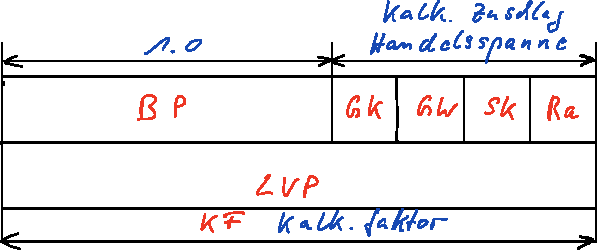
\includegraphics[width=0.6\textwidth]{images/Skizze/03_Kalkulationsfaktor_Skizze.pdf}
\caption{Kalkulationsfaktor}
%\label{fig:}%% anpassen
\end{figure}

\textbf{Kalkulationsfaktor} (KF) wievielmal höher der (Verkaufspreis =
Listenpreis) gegenüber (Bezugspreis) bezieht sich auf das Lager,
Ersatzteil

$\boxed{KF = \frac{LVP}{BP}} \quad \to \boxed{LVP = BP \cdot KF}$

\textbf{Kalkulationszuschlag} enthält
$(GK + \text{Gewinn} + \text{Skonto} + \text{Rabatt})$ bezogen auf
(Bezugspreis)

\textbf{Handelsspanne} (HSP) unterschied zwischen (Verkaufspreis +
Bezugspreis) bezogen auf (Verkaufspreis)
$\boxed{HSP_\% = \frac{HSP \cdot 100}{LVP}}$
$\boxed{HSP_\text{EUR} = LVP - BP}$

\subsubsection{Verkauf von Tauschteilen und
Agenturwarenverkauf}\label{verkauf-von-tauschteilen-und-agenturwarenverkauf}

\textbf{Altteilesteuer} (AT-St) kauft ein Kunde ein Tauschteil und gibt
dabei sein defektes Teil (Altteil) in Zahlung, fällt Altteilesteuer an.
$\boxed{LVP \cdot 10~\% \cdot 19~\%} \quad \boxed{LVP \cdot 0,1 \cdot 0,19}$

\textbf{Agenturwaren} sind Waren, die im Auftrag und auf Rechnung einer
Fremdfirma verkauft werden (Preise inkl. Gesetzl. Ust.).

\subsubsection{Rechnungserstellung}\label{rechnungserstellung}

Kostenvoranschlag (KVA)

\textbf{Formvorschriften beachten}

\begin{itemize}
\item
  Rechnung schriftlich mit Rechnungsnummer und Leistungsdatum
\item
  Kunden- und Fahrzeugdaten wichtige aufführen
\item
  Arbeitspreis und Ersatzteilpreise detailliert aufführen
\item
  Netto-Rechnungsbetrag, Umsatzsteuer, Altteilesteuer und
  Brutto-Rechnungsbetrag einzeln aufführen.
\end{itemize}

$\text{AP} = \text{Flh} \cdot \text{StVs} \quad \text{AP} = \text{AW-Vs} \cdot \Sigma \text{AW}$

$\text{AP}_\text{Seko} = \Sigma \text{AW} \cdot \text{Seko}_{AW} \quad \text{Werkstatt AW-Preis} = \Sigma \text{AW} \cdot \text{Seko}_{AW} + \text{GW}$

\lstset{language=Python}% C, TeX, Bash, Python 
\begin{lstlisting}[
	%caption={}, label={code:}%% anpassen
]
Pos    Bezeichnung                              AW-Vs x AW           Preis
_____________________________________________________________________________
  1
  2
  3
_____________________________________________________________________________
  Summe AP                                                                EUR

                           EK                                  VP
                           80 %  20 %     100 % 24 %           124 %
                           ZEP x Rabatt = LEP + GW                      
Anzahl      Ersatzteil     (EK x 1,25)    (LEP x 1,24)       E-Preis Et-Preis
   oder
Anzahl      Ersatzteil     Rabatt (Kunden)      LVP          E-Preis Et-Preis
_____________________________________________________________________________
  1                        10 %                 (Preis x 0,9)
  1         AT-Teil
  3
_____________________________________________________________________________
  Summe ET                                                                EUR

                                                                     Preis
_____________________________________________________________________________
  AP
+ ET
+ Fremdleistung
+ Zubehör
+ Schmierstoffe
= Reparaturkosten 
+ UST                                           19 % 
+ AT-Steuer (AT-Teil x 0,1 x 0,19)
+ Agenturware (Öl)
_____________________________________________________________________________
= Rechnungsbetrag                                                         EUR
\end{lstlisting}

\newpage

\subsubsection{Kosten des Lagers}\label{kosten-des-lagers}

\begin{itemize}
\item
  Kosten des Lagers
\item
  Kennwerte des Lagers
\end{itemize}

\newpage

\section{Abschreibung}\label{abschreibung}

\begin{itemize}
\item
  linear
\item
  degressiv: am Anfang schnell abschreiben, Investition ankurbeln
\item
  Kombination aus linear und degressiv
\item
  Leistung
\end{itemize}

\textbf{Begriffe}

\begin{itemize}
\item
  Anschaffungswert
\item
  Buchwert
\item
  Nutzungsdauer
\item
  Abschreibungsbetrag
\item
  Abschreibungssatz
\item
  AfA mindert Gewinn, weniger Steuern zahlen
\item
  GWG
\end{itemize}

\textbf{Berechne den Buchwert nach 6 Jahren}

\lstset{language=Python}% C, TeX, Bash, Python 
\begin{lstlisting}[
	%caption={}, label={code:}%% anpassen
]
  Einkaufspreis  10.000,00
+ 5%                500,00   // Transport-, Montage und Anschlusskosten
__________________________
= AK             10.500,00   // ND: 8J

            Jahr Abschreibung Buchwert
__________________________________________           
degressiv 1J 20%     2.100,00 8.400,00 EUR
          2J 20%     1.680,00 6.720,00 EUR
          3J 20%     1.344,00 5.376,00 EUR      
          4J 20%     1.075,20 4.300,80 EUR
linear    5J         1.075,20 3.225,60 EUR
          6J         1.075,20 2.150,40 EUR
\end{lstlisting}

\newpage


	%%%%%%%%%%%%%%%%%%%%%%%%%%%%%%%%%%%%%%%%%%%%%%%%%%%%%%%%%%%%%%%%%%
    % Bibliographie
    \printbibliography[category=cited]
\end{document}
